\chapter{Especificações Técnicas}

Os componentes básicos de um quadro de distribuição são:
\begin{itemize}
\item Dispositivos de proteção: disjuntores (DTM), interruptores diferenciais (IDR) e dispositivo de proteção contra surtos (DPS);
\item Barramentos de interligação fase;
\item Barramento de Neutro;
\item Barramento de proteção
\item Estrutura: caixa com porta, chapa de montagem dos componentes, isoladores, tampa espelho.
\end{itemize}




\section{Condutores elétricos}
Os cabos elétricos utilizados nas instalações devem possuir classe de encordoamento no mínimo 5 ou 6, tanto para os circuitos terminais, quanto para o alimentador do quadro de distribuição QGD1, os cabos dos circuitos terminais deverão ser cabos isolados de PVC (450/750V), nas cores preta, azul, vermelho, branco e ou verde) e unipolar em EPR para o alimentador do quando QGD1.
Todos os condutores deverão seguir a NBR NM 247-3 e possuir o selo do inmetro, todas as seções desses condutores estão descritas na tabela de carga de acordo com os seus respectivos circuitos e deverão ser seguidos.
ATENÇÃO A escolha dos cabos devem ser realizadas conforme a Norma 5410.

\section{Disjuntores}
Os disjuntores devem ser de tensão nominal de serviço Ue = 400V ou superior. Seguir as correntes nominais de atuação de sobrecarga conforme indicado em projeto. As correntes de ruptura devem ser de 3kA para os disjuntores de circuitos terminais e 5kA para o disjuntor geral. As curvas de disparo devem seguir conforme indicado na tabela de carga, assim como a escolha da quantidade de pólos.
Todos os disjuntores existentes no projeto devem ser de fabrincantes que possuem o selo do INMETRO de certificação compulsória e os responsáveis pela compra e execução dos materiais deverão utilizadas marcas de confiança e consolidadas no mercado como Schneider, WEG, ABB, Siemens, Steck ou similar. 
Todos os disjuntores deverão seguir as normas:\begin{list}{•}{•}
\item ABNT NBR 5361 - Disjuntores de baixa tensão;
\item ABNT NBR IEC 60947-2 -  Dispositivo de manobra e comando de baixa tensão;
\item ABNT NBR NM 60898 (ou IEC 61009-2-1) – Disjuntores para proteção de sobrecorrentes para instalações domésticas e similares
\end{list}



\begin{table}[htbp]
\centering
\caption{Capacidade de interrupção máxima $I_{cn}$ }

\begin{tabular}{|l|c|c}
%\begin{tabular}{llccccccccc}

& 127/220 V 220/380 V  \\\hline
NBR NM 60898 & 5kA & 3 kA)\\ \hline
NBR IEC 60947-2 & 5kA & 4,5 kA)\\ \hline
\end{tabular}
\label{tab:disjIcn}
\end{table}



\section{IDR – Interruptor diferencial residual}

Dispostivos DR são seccionadores mecânicos projetados para provocar abertura na ocorrência de uma corrente de fuga à terrra. Tem como principal objetivo proteger as pessoas contra os efeitos dos choques elétricos prejudiciais a saúde. De acordo com NBR 5410/2004 item 5.1.3.2.2, seu uso é obrigatório nos circuitos elétricos localizados em áreas molhadas e externa [Siemens 2023].
Sua versão de corrente residual até 30 mA são destinados a principalmente a proteção de pessoas, acima deste valor, são apropriados para a proteção de instalações elétricas. Existe 3 tipos de dispositivos DR:
    1. Tipo AC – detecta correntes residuais alternadas;
    2. Tipo A – detecta correntes residuais alternadas e continua pulsantes.
    3. Tipo B – detecta correntes residuais alternadas, continuas pulsantes e continuas puras[Siemens 2023].
O IDR a ser utilizado deverá ser ligado em série com o disjuntor geral e este deve possuir corrente nominal igual ou superior a corrente nominal do disjuntor termomagnético geral do quadro QDC. O valor de atuação da corrente diferencial do IDR deverá ser de 30mA. O IDR deverá seguir a norma ABNT NBR NM 61008-1 (verificar validade no site da ABNT)
\section{DPS – Dispositivo de proteção contra surtos elétricos}
O DPS utilizado deverá ser do tipo classe II, 175V e 20kA e este deverá ser instalado dentro do quadro de distribuição QGD1. O DPS deverá seguir a norma ABNT NBR IEC 61643-1 (verificar validade no site da ABNT), NBR 5410 e NBR 5419.

\section{Quadro elétrico e acessórios}
    1 O quadro de distribuição deve seguir a norma NBR IEC 60439-1 e NBR 5410.

No quadro deverão estar presentes os seguintes itens:

    2 Tensão nominal: (220/127V)
    3 Corrente de demanda: 34,55A
    4 Capacidade de Curto-circuito: 5kA
    5 Grau de proteção IP adequado e no mínimo IP2X.
    6 Placa de Identificação do quadro contendo nome ou marca do fabricante e tipo ou numero de identificação.

O instalador deverá inserir etiqueta de advertência conforme NBR 5410 no item 6.5.4.10 mostrada abaixo:

5.6.5.2 Quando existir risco de choque elétrico, o dispositivo de seccionamento de emergência deve seccionar todos os condutores vivos, observada a prescrição de 5.6.2.2
Perfil
Canaleta DN
as canaletas DN servem para agrupar, proteger e organizar os fios e cabos dentro do quadro elétrico. São de PVC rígido em conformidade com a Norma Diretiva 2002/95/EC-RoHS

\subsection{Grau de Proteção}
Determina a proteção do quadro metálico quanto a entrada de corpos estranhos e penetração de água por frestas e orificios do quadro. As normas especificam os graus de proteção por código IPXY, onde X indica o grau de proteção quanto à penetreção de corpos sólidos e contatos acidentais. Enquanto que o Y é um número que indica o grau de proteção quanto a penetração de água internamente no quadro quando fechado. 
Os graus de proteção identificados pelas letras IP seguida de dois números que significam (%\citep{Filho2013})

\begin{itemize}
\item \textbf{Primeiro algarismo}
 	\begin{description}
 	\item[0-] sem proteção;
 	\item[1-] corpos estranhos com dimensões acima de 50 mm;
 	\item[2-] corpos estranhos com dimensões acima de 12 mm;
 	\item[3-] corpos estranhos com dimensões acima de 2,5 mm;
 	\item[4-] corpos estranhos com dimensões acima de 1 mm;
 	\item[5-] proteção contra acúmulo de poeira prejudicial ao equipamento;
 	\item[6-] proteção contra penetração de poeira.
 	\end{description}
 	
 \item \textbf{Segundo algarismo}
 
 		\begin{description}
 		\item[0-] sem proteção;
 		\item[1-] pingos de água na vertical;
 		\item[2-] pingos de água até a inclinação de 15° com a vertical;
 		\item[3-] água de chuva até a inclinação de 60° com a vertical;
 		\item[4-] respingos em todas as direções;
 		\item[5-] jatos de água em todas as direções;
 		\item[6-] imersão temporária;
 		\item[7-] imersão;
 		\item[8-] submersão.
 		\end{description}
\end{itemize}



\subsection{Bornes}
Os bornes permitem uma conexão segura quadro a rede e ao Painel. Propocionando flexibilidade, facilidade e rapidez na instalação. Existe três opções de conexão: por parafuso, por mola e plug-in.

\begin{figure}[h]
    \centering
    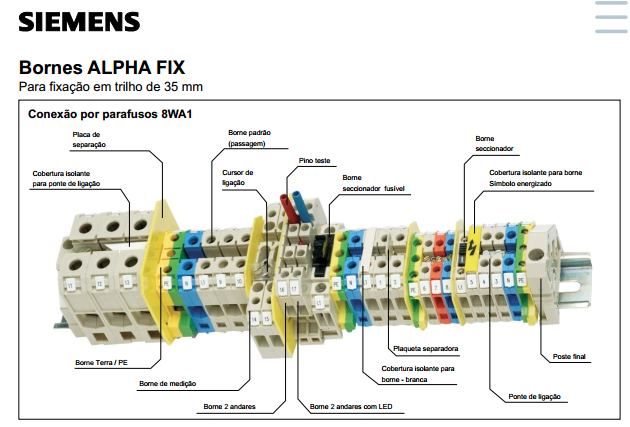
\includegraphics[width=0.6\textwidth]{image/BORNESIMENS.png}
    %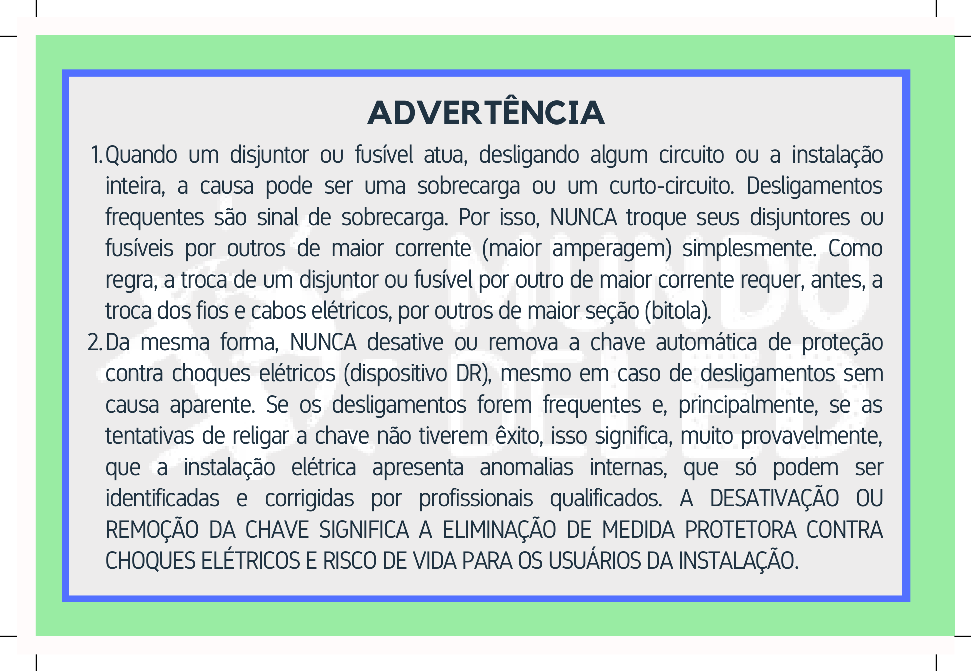
\includegraphics[width=4cm]{image/EtiqAdvQD.pdf}
    \caption{Imagens retirada do catálogo siemens com vários tipos de borne}
   \label{fig:bornes}
\end{figure}
\begin{description}
\item[Borne padrão] utilizado como um conector de passagem, tem disponivel em vários tamanho, cores em geral bege, azul e laranja. Servirão para conectar condutores de fase e neutro de entrada e saída do quadro.
\item[Borne Terra] borne especial para proteção equipotecial, sempre na cor verde-amarela. Por suas caracteristicas, nunca deve ser utilizado como borne de passagem padrão. Ou seja, SOMENTE utilizar como entrada ou saida de aterramento, NUNCA ligar condutores fase ou neutro.
\end{description}
\subsection{Barramentos}
Os barramentos de cobre são indicados para instalações elétricas com o objetivo de fazer a ligação de vários circuitos, de modo mais funcional e seguro.
O barramento fase tipo pente ou pente de conexão ou barramento de alimentação tem modo de montagem horizontal em linha. Serva para ligações monofásicas, bifásicas e trifásicas. Com corrente nominal de 63 A a 130 A, podem ser encontrados com 12, 24 e 57 polos. Tem capa ou terminal isolador apropriado, onde uma peça tem cinco módulos isolador. 
\begin{figure}
\centering
\begin{subfigure}{0.4\textwidth}
	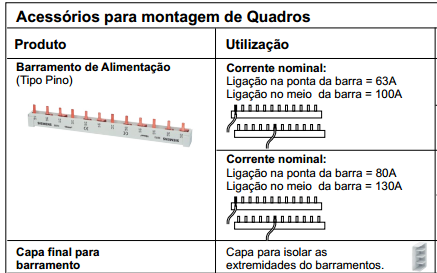
\includegraphics[width=\textwidth]{image/barramentofase.png}
	\caption{Barramento fase tipo pente e seu modo de ligação e respectiva corrente nominal. }
	\label{fig:advQD_1}
\end{subfigure}
\hfill
\begin{subfigure}{0.4\textwidth}
    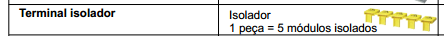
\includegraphics[width=\textwidth]{image/barramentocapa.png}
    \caption{Capa isolante}
    \label{fig:advQD_2}
\end{subfigure}
\caption{Barramento para fase caracteristicas retirado do catálogo Simens}
\label{fig:advQD}
\end{figure}

\section{Dispositivos de comando}
\subsection{Contatores}
Contatores são elementos de comandos eletromêcanicos, que permite o controle de correntes elevadas por meio de circuitos de baixa corrente. O contator funciona como uma chave eletromagnética, constituido por uma bobina, que quando alimentada, cria um campo eletromagnetico que fecha o circuito, e ao cessar a alimentação da bobina o circuito é aberto. 
%
\begin{figure}[h]
    \centering
    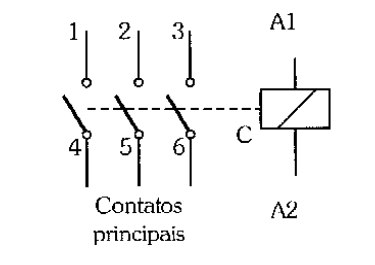
\includegraphics[width=0.6\textwidth]{image/contator_simbolo.png}
    
    \caption{Simbologia do contator. Fonte\cite{Franchi2008}}
   \label{fig:bornes}
\end{figure}

\subsection{Interruptor horário}
Interruptor horário eletrônicos ou interruptor temporizador, permite a programação de horário para ligar e desligar automáticamente, com algumas combinações de frequência diária semanal, como por exemplo, todos os dias, dias úteis, entre outras.
A Figura \ref{fig:esqtemp_1} tem o esquema de ligação para controle automático de luminosos, um sistema por comando direto, e outro com uso de contator necessário para circuitos luminosos com corrente acima de 10 A. Assim como os interruptores a capacidade nominal de o interruptore temporizador é de 10 A.
\begin{figure}
\centering
	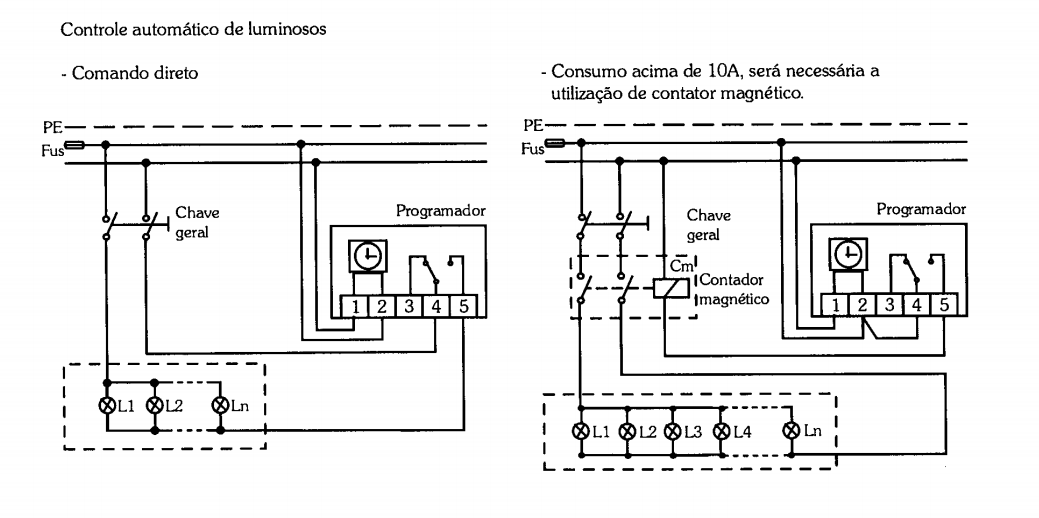
\includegraphics[width=\textwidth]{image/esqTemp.png}
	\caption{Esquema multifilar de ligação do controle automático por interruptor temporizador.}
	\label{fig:esqtemp_1}
\end{figure}


\subsection{Relé de Impulso}
Possivel comandar com botão pulsador a distância ou por um ou mais pulsadores, para os esquemas multifilar mostrados nesta seção, considerar a carga de iluminação dentro da capacidade do relé.
